% https://pt.sharelatex.com/learn/Sections_and_chapters

\documentclass[graduacao,brazil]{ThesisPUC}
\usepackage{float}
\usepackage{enumerate}
\usepackage[final]{pdfpages}

%%%%%%%%%%%%%%%%%%%%%%%%%%%%%%%%%%%%%%%%%%%%%%%%%%%%%%%%%%%%%%%%%%%%%%%%%%%%%%%%

\newcommand{\Rset}{\mathbb{R}}
\newcommand{\Zset}{\mathbb{Z}}

%%%%%%%%%%%%%%%%%%%%%%%%%%%%%%%%%%%%%%%%%%%%%%%%%%%%%%%%%%%%%%%%%%%%%%%%%%%%%%%%

\autor{Julio Ribeiro da Silva}
\autorR{Ribeiro da Silva, Julio}
\orientador{S\'{e}rgio Lifschitz}
\orientadorR{Lifschitz, S\'{e}rgio}

\titulo{PrISMA}
\titulouk{PrISMA}
\subtitulo{Programa de Instru\c{c}\~{a}o \`{a} Solicita\c{c}\~{a}o de Matr\'{i}cula Acad\^{e}mica}
\dia{19} \mes{Novembro} \ano{2014}

\cidade{Rio de Janeiro}
\CDD{510}
\departamento{Inform\'atica}
\programa{Engenharia da Computa\c{c}\~{a}o}
\centro{Centro T\'{e}cnico Cient\'{i}fico}
\universidade{Pontif\'{i}cia Universidade Cat\'{o}lica do Rio de Janeiro}
\uni{PUC--Rio}
\course{Engenharia da Computa\c{c}\~{a}o}
\diploma{Bacharel em Engenharia da Computa\c{c}\~{a}o}

%%%%%%%%%%%%%%%%%%%%%%%%%%%%%%%%%%%%%%%%%%%%%%%%%%%%%%%%%%%%%%%%%%%%%%%%%%%%%%%%

  \agradecimentos{%
Primeiramente, à minha família, que esteve comigo durante todos os momentos da minha vida e tornaram possível eu chegar até aqui.

Em segundo lugar à Luiza Noronha, que foi quem esteja ao meu lado durante todo o desenvolvimento deste projeto. Assim como meu orientador Sérgio Lifschitz, a quem eu atribuo a autoria da ideia, e que também tornou a sua implantação possível.

Ao Waldecir Vicente Faria e Victor Paulo Tolini Málaga, que fizeram parte do meu grupo de Banco de Dados I, que foi onde surgiu a primeira versão do projeto. Ao João Alexandre, Diego Malone e Frederico Barnard, que também deram suas valiosas contribuições no desenvolvimento.

Ao professor Washington Braga, que foi quem apresentou o problema e sempre acreditou e defendeu o sistema, ajudando inclusive na sua divulgação para todos os alunos da PUC-Rio. E também à equipe do SAU (Sistema Acadêmico Universitário), que disponibilizou todos os dados necessários a sobrevivência do sistema.

Ao professor Luiz Fernando Bessa Seibel, que me acolheu em seu laboratório por pouco mais de três anos e sempre acreditou em mim.

À todos aqueles que estiveram ao meu lado durante toda a fase da graduação e que me ajudaram a superar os desafios, que estiveram sempre estiveram ao meu lado. Tanto as novas, quantos as velhas amizades que foram estabelecidas.

E, não menos importante, à todos os alunos da PUC-Rio que utilizaram o PrISMA. Sem vocês o projeto não teria o sucesso que foi alcançado.
}


%%%%%%%%%%%%%%%%%%%%%%%%%%%%%%%%%%%%%%%%%%%%%%%%%%%%%%%%%%%%%%%%%%%%%%%%%%%%%%%%

 \chaves{%
   \chave{Banco de dados}%
   \chave{Experi\^{e}ncia do usu\'{a}rio}%
   \chave{Aplica\c{c}\~{a}o web}%
   \chave{API REST}%
   \chave{PrISMA}%
 }
 
 \resumo{
Na PUC-Rio, no início de cada período os alunos informam quais turmas gostariam de cursar, de acordo com os seus planejamentos. No entanto, dado que o número de vagas por turmas é limitado, na maior parte das vezes não é possível atender a todos os pedidos de todos os alunos. Este problema que o PrISMA se propõe a minimizar. Através de uma aplicação web bastante poderosa, e ao mesmo tempo de fácil uso, auxiliar os alunos passo a passo nas suas decisões na hora de montar o seu planejamento de turmas para o período seguinte.
 }
 
 
% %%%%%%%%%%%%%%%%%%%%%%%%%%%%%%%%%%%%%%%%%%%%%%%%%%%%%%%%%%%%%%%%%%%%%%%%%%%%%%%%
 
 \chavesuk{
   \chave{Database}%
   \chave{User Experience}%
   \chave{Web application}%
   \chave{REST API}%
   \chave{PrISMA}%
 }
 
 \resumouk{%
At PUC-Rio, in the beginning of each period students tells which classes they would like to attend, according to their schedules. However, given that the number of vacancies for classes is limited, in most cases it is not possible to attend all requests for all students. This is the problem PrISMA aims to minimize. Through a very powerful and easy to use web application assist students step by step in their decisions when scheduling classes for the following period.
 }


%%%%%%%%%%%%%%%%%%%%%%%%%%%%%%%%%%%%%%%%%%%%%%%%%%%%%%%%%%%%%%%%%%%%%%%%%%%%%%%%

\modotabelas{fig} % nada, fig, tab ou figtab

%%%%%%%%%%%%%%%%%%%%%%%%%%%%%%%%%%%%%%%%%%%%%%%%%%%%%%%%%%%%%%%%%%%%%%%%%%%%%%%%

\begin{document}

\chapter{Introdução}

As universidades de forma geral adotam modelos muito parecidos para que alguém consiga conquistar um diploma de graduação. Para este projeto, o modelo utilizado como referência foi aquele adotado pela Pontifícia Universidade Católica do Rio de Janeiro (PUC-Rio). Todos os conceitos aqui abordados estarão condicionados neste contexto, apesar de que nada impede que possam ser extendido para as demais universidades.

Para se cumprir um curso de graduação, disciplinas obrigatórias, eletivas e algumas outras atividades devem ser devidamente cumpridas. Como este conjunto de disciplinas é bastante extenso, e existe uma série de pré-requisitos necessários a serem cumpridos para aquelas disciplinas mais avançadas, naturalmente demora alguns anos para se conseguir o diploma.

Pré-requisitos são restrições impostas às disciplinas com o objetivo de nivelar o conhecimento dos alunos que irão cursá-la. Dessa maneira, é facilitado o trabalho do professor, que por sua vez pode assumir que parte da matéria já faz parte do conhecimento dos alunos. Logo, período a período, o conjunto de disciplinas que os alunos podem, de fato, cursar é limitado em apenas uma fração delas.

Diversas outras restrições também existem ao se solicitar uma disciplina para o período conseguinte. Como, por exemplo, o somatório final de créditos de cada disciplina não deve ser superior a 30, naquele período. Caso o aluno tenha tido algum baixo desempenho no período anterior, essa quantidade pode ser ainda menor.

As disciplinas, por sua vez, são representadas por turmas na hora que os alunos montam os seus horários. Ou seja, como cada disciplina possui uma ou mais turmas, os alunos solicitam as turmas, não disciplinas. Cada turma possui um horário e professor associado. Dessa maneira, preferencias pessoais por parte dos alunos por horários ou professores contribuem mais ainda para a complexidade das escolhas na hora do planejamento.

A PUC-Rio organiza seu processo de inscrição em turmas em 3 etapas. Na primeira o aluno solicita uma grade completa, com todas as turmas que gostaria de cursar. Passada essa etapa o aluno tem mais 2 outras etapas para ajustar a sua grade, caso tenha perdido a primeira etapa ou queira simplesmente realizar alguma alteração na solicitação anterior. São as chamadas etapas de ajuste de De-Para. Em todas as etapas o processo é realizado online, através do sistema PUC-Online. A última, por ser definitiva, também pode ser realizada presencialmente.

E foi esse o contexto exposto pelo professor Washington Braga, responsável pela Diretoria de Admissão e Registro da PUC-Rio, quando eu ainda cursava Banco de Dados I no segundo semestre do ano de 2010, ministrada pelo professor Sérgio Lifschitz, meu atual coordenador. Segundo o Washington, a quantidade de alunos que restava até a última etapa de ajuste, presencialmente, era muito grande. Dessa forma, muitos recursos deveriam ser alocados pela universidade para resolver este problema e poucos alunos ficavam realmente satisfeitos.

O meu orientador, naquela época, já havia pensado sobre o problema e mostrou como ele, na sua época, se organizava para escolher suas turmas. Ele se reunia com os seus colegas em uma sala da faculdade, desenha no quadro uma tabela semanal de horários e ali ia combinando as turmas até encontrar a combinação que melhor atendesse a todos. E algo similar eu e meus amigos também fazíamos. Só que ao invés de quadro utilizávamos o Excel, e ao invés de nos reunirmos em uma sala utilizávamos a internet para compartilhar nossos horários, até encontrarmos aquele comum à todos.

E esse foi o conceito inicial utilizado pelo meu grupo na disciplina, composto também por Waldecir Vicente Faria e Victor Paulo Tolini Málaga. O protótipo apresentado foi muito bem aceito pelo Sérgio, que logo propôs tornar o sistema disponível para todos.

A equipe foi então reorganizada, passando a ser composta por mim, Luiza Noronha, João Alexandre e Diego Malone. Adicionamos tela de login e tela de cadastro. Entramos em contato com a equipe do Sistema Universitário Acadêmico (SAU) para disponibilizar os dados dos alunos que utilizariam o PrISMA. Mas, para aquele momento, foi disponibilizado individualmente para cada aluno um arquivo XLS que viria a ser utilizado no cadastro do nosso sistema.

O sistema, do jeito que estava, já era muito útil, principalmente pelo fato de já implementar algumas restrições, as quais os alunos não precisariam mais se preocupar, e por apresentar todos os dados necessários para o planejamento em apenas um sistema. Anteriormente era necessário acessar diversos sites diferentes para se acessar todos os dados.

Muitas críticas, muitos elogios, mudanças lá e cá no sistema. Contamos com a ajuda do Frederico Barnard Ferreira em um dado momento do sistema. Até o momento em que sobrou apenas eu e a Luiza. Naquele ponto já havíamos adquirido certa experiência em desenvolvimento WEB e não estávamos mais satisfeitos em manter aquele código. Foi aí então que decidimos remodelar o sistema do zero. Naquela época conhecemos um grupo do curso de designer que recentemente havia acabado de apresentar um trabalho conceitual acerca do mesmo tema. O grupo era composto por Gabriel Martinelli, Denis Neves, Glauber Borges e Maurício Fragale. E logo notamos que tanto o conceito quanto a versão do PrISMA naquela época se completavam. O desafio era como encaixar os blocos. Depois de muitas reuniões chegamos em um consenso e, eu e Luiza, realizamos a implementação.

Diversas novas funcionalidades foram implementadas. Foi feito um acordo com o SAU para disponibilização dos dados dos alunos diretamente para o PrISMA (mediante termo de confidencialidade), ao invés dos alunos terem que entrar manualmente com os seus dados. E os alunos agora poderiam usar suas próprias credenciais do PUC-Online, evitando assim a etapa de cadastro.

O sucesso dessa vez, foi muito mais expressivo. Chegando na casa dos milhares de acessos, e diversos elogios. Inclusive, algum tempo depois, o PrISMA foi utilizado como referência para o novo sistema de entrada de dados da PUC, que mudou bastante da última versão para a atual.

Por mais que a última versão do PUC Online tenha mudado conceitualmente, o PrISMA, da maneira que foi modelado pela última vez, continua sendo extremamente útil para a etapa que antecede a primeira etapa de matrícula. A ferramenta desenvolvida continua extremamente rica em funcionalidade e muito útil para aqueles que desejam se planejar com antecedência.

%%%%%%%%%%%%%%%%%%%%%%%%%%%%%%%%%%%%%%%%%%%%%%%%%%%%%%%%%%%%%%%%%%%%%%%%%%%%%%%%

\chapter{Estado da Arte} % problema a ser resolvido

A PUC-Rio tem a sua própria forma de organizar a inscrição dos alunos nas turmas, o que mudou desde a primeira versão do PrISMA. No entanto, alguns conceitos permanecem.

O principal conceito é o de ranking de alunos. Esse ranking é necessário na hora de dizer quais alunos têm prioridade na hora de escolher determinada turma. Ele é definido a partir das informações de C.R. (coeficiente de rendimento) acumulado e da quantidade de créditos totais cumpridos, em relação à todos os períodos.

Dificilmente os alunos melhores classificados não terão suas solicitações atendidas. Mas os demais devem estar cientes da sua condição e serem mais cautelosos ainda nos seus planejamentos. Quando isso não acontece, solicitando turmas muito concorridas, por conta de preferência de horários ou de professores, dificilmente suas solicitações serão atendidas, afastando ainda mais o resultado esperado do real alcançado.

Abaixo será explicado como funcionava a versão antiga do PUC Online, que era a utilizada quando se começou a implementar o PrISMA, e como funciona atualmente a última versão, que está bem mais parecido com a última versão do sistema.

Vale notar que apenas a primeira etapa de matrícula será abordada neste relatório por ser o foco do problema. Mas nada impede que o PrISMA também seja utilizado nas demais etapas como ferramenta de auxílio.

\section{PUC Online Antigo}

O sistema antigo para entrada dos dados era composto apenas por uma tela e, basicamente, uma tabela. As três colunas representam a primeira, segunda e terceira opção de escolhas e as linhas as escolhas de turmas em si. E em cada célula é possível entrar com qualquer turma, mesmo que não seja possível ser cursada.

\begin{figure}[H]
    \centering
    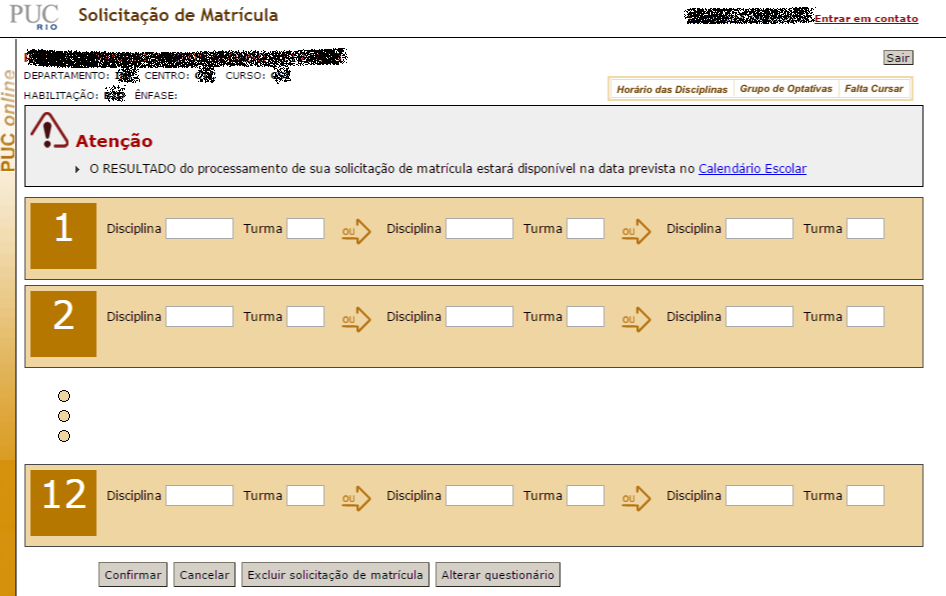
\includegraphics[width=\linewidth]{img/puc_online_antigo.png}
    \caption{Interface antiga do PUC Online.}
\end{figure}

Idealmente, as segundas e terceiras opções devem ser turmas ou da mesma disciplina ou do mesmo horário daquela preenchida na opção anterior, na mesma linha. Dessa forma, atuando realmente como uma opção caso não tenha sido possível se matricular na turma anterior. No entanto, isso nos leva a diversas consequências, como iremos analisar.

A ordem de processamento do algoritmo utilizado sobre a tabela é a seguinte:

\begin{enumerate}

	\item Inicia procedimento na primeira linha e primeira coluna.

	\item Verifica se não existe turma da disciplina corrente cadastrada.

	\item Verifica se a disciplina corrente atende todos os pré-requisitos.

	\item Verifica se o horário referente a turma solicitada ainda não está preenchido.

	\item Verifica se ainda há vaga na turma solicitada.

	\item Condições anteriores atendidas?

	\begin{enumerate}

		\item  Sim. Então matricula turma e pula para a próxima linha. 

		\item  Não. Existe mais opção para esta linha?

		\begin{enumerate}

			\item Sim. Pula para a próxima opção.

			\item Não. Pula para a próxima linha.

		\end{enumerate}


	\end{enumerate}

	\item Retorna ao passo 2 e repete o processo, até que acabem as disciplinas ou atinja a quantidade máxima de créditos que pode ser cursada no período.

\end{enumerate}

Como é possível perceber, por exemplo, se uma turma na primeira opção for devidamente atendida, todas aquelas que estão listadas nas próximas opções na linha corrente serão ignoradas. Um problema causado por esse comportamento está quando o aluno não entende corretamente o conceito de opção e coloca todas as turmas a serem solicitadas na mesma linha, mesmo quando elas não têm relação alguma.

Outro problema se encontra na prioridade natural entre as linhas da tabela de solicitação, provocando, muitas das vezes, consequências indesejadas. Por exemplo, caso na primeira linha seja escolhida a segunda opção que, por acaso, se encontra no mesmo horário da primeira opção da linha debaixo, não será possível se cadastrar nessa última por conta de horário já preenchido.

Esse é um tipo de cascata que torna o correto preenchimento dessa tabela um grande desafio, principalmente para aqueles que não estão muito bem classificados segundo o ranking da PUC. Aqueles que estão melhor classificados não precisam nem preencher as demais opções. Preencher o primeiro campo de cada linha que na grande maioria das vezes não trará problemas.

Nesta primeira etapa, esse sistema ficava aberto por um determinado tempo para que todos os alunos pudessem se organizar e realizar suas solicitações. Durante esse tempo, nenhuma ferramenta de auxilio era oferecida, forçando o aluno a buscar as turmas que estava sendo oferecidas em lugar (chamado de Micro-Horário), a lista de disciplinas que devem ser cursadas (chamada de Falta-Cursar) em outro, a ementa e pré-requisitos referente a cada disciplina em outro, para então realizar a solicitação em um último lugar diferente dos demais. Muito trabalho que, por mais importante que fosse, nem todos se despunham a ter.

Após a primeira etapa, executava-se o algoritmo exposto acima e divulgava-se o resultado final para cada aluno. Inclusive críticas simples que podem ter sido feito anteriormente, como checagem de pré-requisitos, só eram feitas após o processamento final. As próximas etapas de ajuste que não serão abordados nesse relatório.


\section{PUC Online Novo}

Recentemente a equipe do SAU (Sistema Acadêmico Universitário) liberou a nova versão do seu sistema de solicitação de turmas. Não apenas o sistema, mas o modelo utilizado como um todo também foi modificado.

\begin{figure}[H]
    \centering
    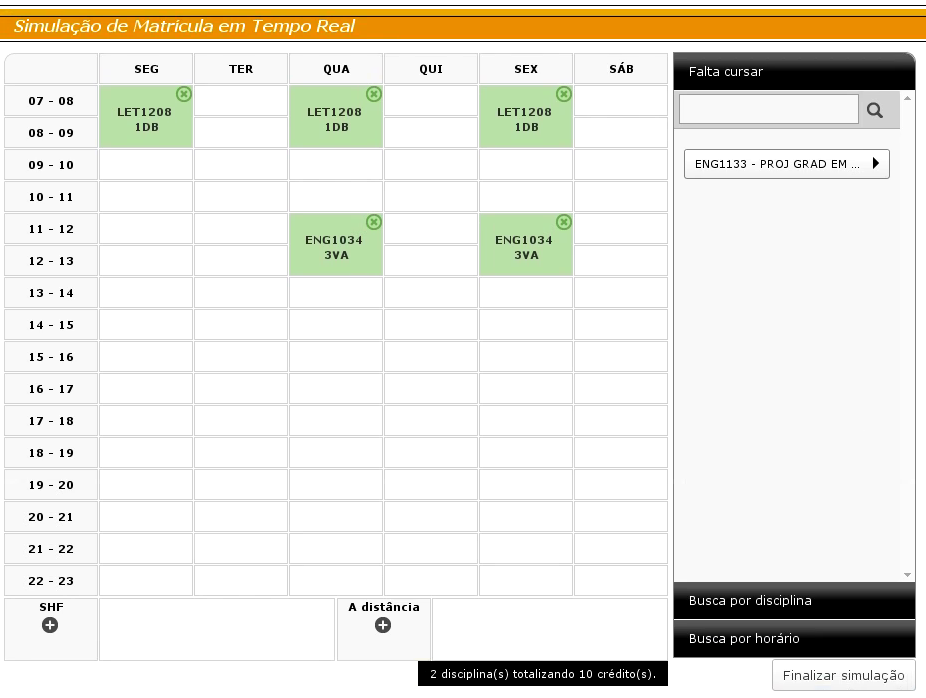
\includegraphics[width=\linewidth]{img/puc_online_novo.png}
    \caption{Interface nova do PUC Online.}
\end{figure}

Ao invés de ter uma janela de tempo em que todos os alunos podem entrar no sistema de uma única vez, e ao final do prazo o sistema fazer o processamento e dizer quais solicitações foram de fato atendidas, agora cada grupo de alunos é alocado em uma janela de horários de 2 horas para que possa fazer sua solicitação, em uma interface de entrada de dados parecida com a última versão do PrISMA. Esse sistema é chamado de Matrícula em Tempo Real.

A grande vantagem é que uma vez selecionada a turma, o aluno já estará matriculado e com a sua vaga garantida. Podendo assim tentar todas as possibilidades na mesma hora que estiver se planejando. Ou seja, no decorrer dessa etapa as turmas já estarão sendo preenchidas e, os próximos alunos a acessarem o sistema, que tem menor prioridade, já terão seu conjunto de escolha de disciplinadas reduzido.

Uma grande desvantagem está no fato de que cada aluno tem uma janela de tempo muito curta para acessar o sistema. Caso ele perca seu horário, no final do seu respectivo dia ele pode acessar novamente, mas terá sua prioridade reduzida, pois alunos com prioridades menores já terão acessado o sistema.

No entanto, esse novo sistema foi uma grande evolução. Agora todos os dados necessários à matrícula são apresentados no mesmo lugar. Isto é, é possível verificar quais disciplinas que deve-se cursar para completar o curso (Falta-Cursar), assim como procurar por toda as turmas que estão sendo oferecidas no período de maneira muito simples, inclusive clicando nas células na tabela de horários na esquerda, procurando assim por turmas naquele respectivo horário. Da mesma forma que foi modelado na última versão do PrISMA.

Mas esse novo sistema por mais intuitivo e fácil de usar que seja, não pode ser acessado antes da janela de horário disponibilizada ao aluno, eliminando assim o seu poder para o plenejamento. Dessa forma, por mais que o PrISMA atual esteja modelado para trabalhar com o sistema antigo do PUC Online, ele continua sendo extremamente útil na etapa anterior à primeira etapa de matrícula.


%%%%%%%%%%%%%%%%%%%%%%%%%%%%%%%%%%%%%%%%%%%%%%%%%%%%%%%%%%%%%%%%%%%%%%%%%%%%%%%%

\chapter{Solução proposta}

Com isso propõe-se o PrISMA. Um sistema Web que começou a ser desenvolvido no segundo semestre do ano de 2010, para disciplina de Banco de Dados I, ministrada pelo meu atual coordenador, Sérgio Lifschitz.

Antes que existisse qualquer sistema de apoio à solicitação de matrícula, eu e alguns amigos já utilizávamos o Excel para nos organizarmos. Era montada uma tabela de horários semanais, ao lado de uma lista de turmas, relacionadas com as suas respectivas disciplinas, horários e professores. Dessa forma, manualmente, as combinações iam sendo feitas na própria planilha, até que o horário que melhor atendesse fosse encontrado.

E essa foi a principal motivação do sistema como um todo. Uma página Web, que poderia ser acessada a qualquer momento, inclusive no meio do período letivo, onde o aluno teria todos os seus dados a mão para que pudesse se planejar melhor. Da mesma maneira, seriam oferecidas diversas funcionalidades para que todo o processo fique mais simples.

Por outro lado, esse sistema seria de grande interesse para a universidade, dado que também poderia ser utilizado pelos coordenadores de departamentos, que gerenciam a disponibilidade de turmas e professores, a terem indicadores com maior confiança quanto à demanda por disciplinas, horários e professores específicos, podendo atender assim a mais alunos.

Indo um pouco mais além, poderia haver um acompanhamento do desempenho dos alunos durante o semestre, avaliando estatisticamente sua probabilidade de conclusão das disciplinas e de quais ele poderá, ou teria interesse, de cursar no próximo semestre. Dessa forma, seria mais um indicador de demanda para os coordenadores. No entanto, essa seria uma funcionalidade que necessitaria de grande integração com o sistema atual da PUC-Rio.

Vale ressaltar que toda modelagem aqui abordada foi feita referenciando sempre o sistema do PUC Online, onde é feita a matrícula. No entanto, nada impede que as mesmas ideias sejam utilizadas em contextos de outras universidades.


\section{Versão alpha}

Essa versão se refere àquela entregue como projeto final da disciplina de Banco de Dados I. Os dados aqui utilizados foram cedidos pelos próprios integrantes do grupo que apresentou este trabalho.

O sistema era composto basicamente por duas telas. Na primeira era apresentada uma lista com todas as disciplinas pertencentes ao fala-cursar do aluno. Da mesma maneira, visando desde já facilitar a facilidade no acesso às informações, cada disciplina acompanhava a referência para sua página oficial, onde é possível verificar sua ementa e pré-requisitos.

\begin{figure}[H]
    \centering
    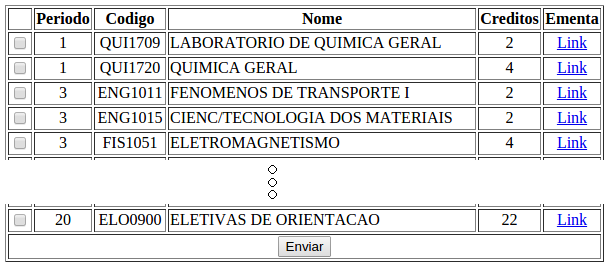
\includegraphics[width=0.7\linewidth]{img/v1_p1.png}
    \caption{Primeira tela da primeira versão.}
\end{figure}

Na segunda tela do sistema, todas as turmas daquelas disciplinas selecionadas são carregadas automaticamente, preenchendo tanto a tabela de horários quanto a lista de disciplinas. Também é possível adicionar mais disciplinas, em caso de eletivas por exemplo, através do código no campo logo abaixo da lista de disciplinas, no canto inferior direito.

\begin{figure}[H]
    \centering
    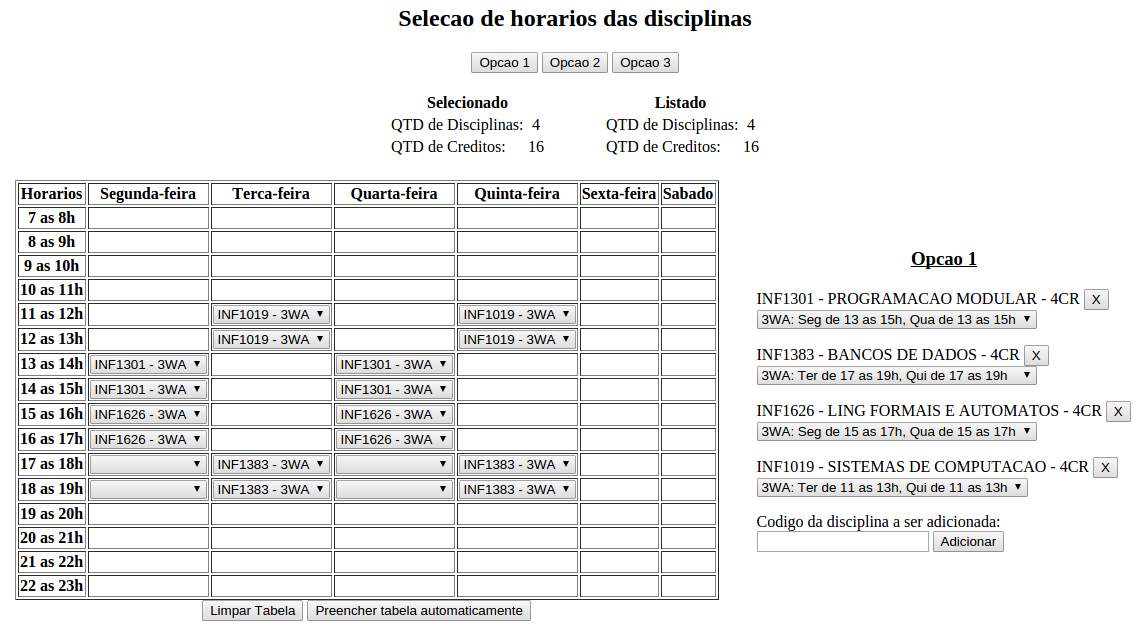
\includegraphics[width=\linewidth]{img/v1_p2.png}
    \caption{Segunda tela da primeira versão.}
\end{figure}

Cada célula da tabela que apresentasse um campo de seleção significava que uma turma das disciplinas selecionadas pode vir a ocupar aquele horário. Ao clicar no campo de seleção e selecionar a turma desejada para aquele horário, na respectiva disciplina, na lista de disciplinas lateral, o campo de seleção de turma daquela disciplina específica também será atualizado.

Quando uma turma selecionada colide em horário com outra turma previamente selecionada, o sistema não deixa a operação ser concluída, avisando o ocorrido. Da mesma forma, caso uma turma referente a uma disciplina tiver sido selecionada, quando outra turma dessa mesma disciplina já tiver sido previamente selecionada, o sistema impedirá a operação, notificando o ocorrido.

Dessa forma, disciplinas podem ser adicionadas e removidas dinamicamente. Turmas podem ser combinadas a vontade, descrevendo exatamente aquele comportamento previamente citado que era realizado no Excel.

No entanto, já nesta versão, visando auxiliar o aluno no primeiro momento do seu planejamento, era oferecido a funcionalidade de preencher a tabela automaticamente. Neste caso, trata-se de um algoritmo guloso que tenta encaixar todas as turmas de todas as disciplinas, uma a uma, até que nenhuma colida em horário, nem se repita disciplina. Ou seja, a primeira combinação encontrada que atenda esses requisitos era apresentada como solução.

Em suma, já nesta versão os alunos têm todos os dados a mão e uma rápida e clara visualização de como as turmas estão sendo combinadas. Levando em consideração, inclusive, algumas críticas mais básicas, como conflitos de horários entre turmas e repetição de turmas de uma mesma disciplina.


\section{Versão beta}

Esta versão se trata de uma atualização daquela exposta anteriormente. Desta vez disponível para utilização por parte de todos os alunos da universidade.

Para isso, foi necessário desenvolver os demais itens que cercam a funcionalidade principal. O principal deles se trata do controle de acesso e carregamento dos dados de cada aluno no sistema.

Infelizmente, naquela época, não foi possível realizar a importação dos dados diretamente do SAU. No entanto, foi disponibilizada uma nova funcionalidade no PUC Online que permitiu baixar em um arquivo todos os dados necessários pelo PrISMA, de forma que, com esse arquivo pudesse ser verificada a autenticidade de quem emitiu, no caso o PUC Online, e assim permitir o cadastro dos alunos no PrISMA. Conforme pode ser visto na imagem que segue.

\begin{figure}[H]
    \centering
    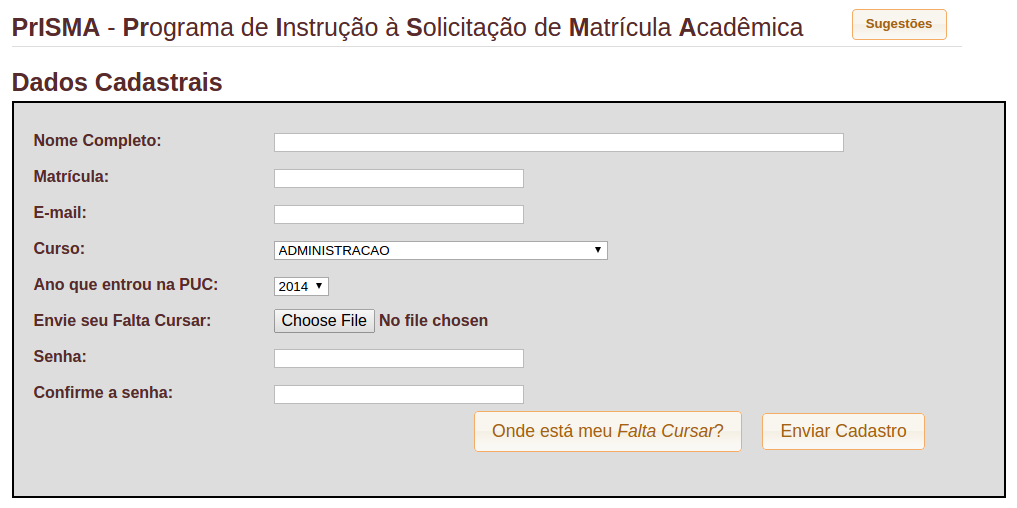
\includegraphics[width=\linewidth]{img/v2_cadastro.png}
    \caption{Tela de cadastro.}
\end{figure}

Esse arquivo contém apenas o falta-cursar do aluno. Ainda não tinha acesso ao histórico, para que pudesse verificar os pré-requisitos das disciplinas. Assim como também não se tinha a informação de quais disciplinas estavam sendo cursadas no momento, para que pudesse avisar o usuário na interface do sistema.

Após feita autenticação no sistema, abre-se então a página principal. Nela é possível selecionar um dos 3 modos de operação do sistema (na última versão deste sistema esses modos não estavam funcionando corretamente).

\begin{figure}[H]
    \centering
    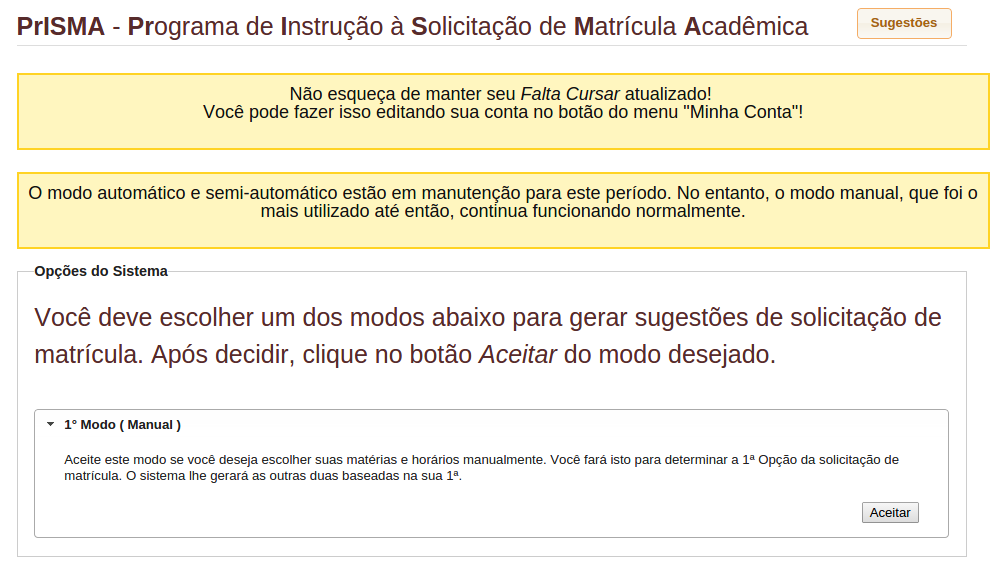
\includegraphics[width=\linewidth]{img/v2_main.png}
    \caption{Tela de entrada no sistema.}
\end{figure}

No modo automático, o próprio sistema escolhe quais disciplinas serão incluídas e qual a combinação de turmas que será utilizada. Para a escolha inicial das disciplinas é utilizada a heurística de se pegar aquelas que, segundo o falta-cursar, devem ser cursadas nos primeiros períodos, e tantas quantas não estourem o limite de 30 créditos. Para a combinação das turmas dessas disciplinas é utilizado o mesmo algoritmo descrito na versão anterior do sistema, onde se escolhe a primeira combinação encontrada, segundo alguns critérios.

No modo semi-automático o aluno escolhe as disciplinas, e na segunda etapa é executado o algoritmo guloso descrito anteriormente. E no modo completamente manual, executam-se as mesmas duas etapas presentes na versão anterior do sistema.

\begin{figure}[H]
    \centering
    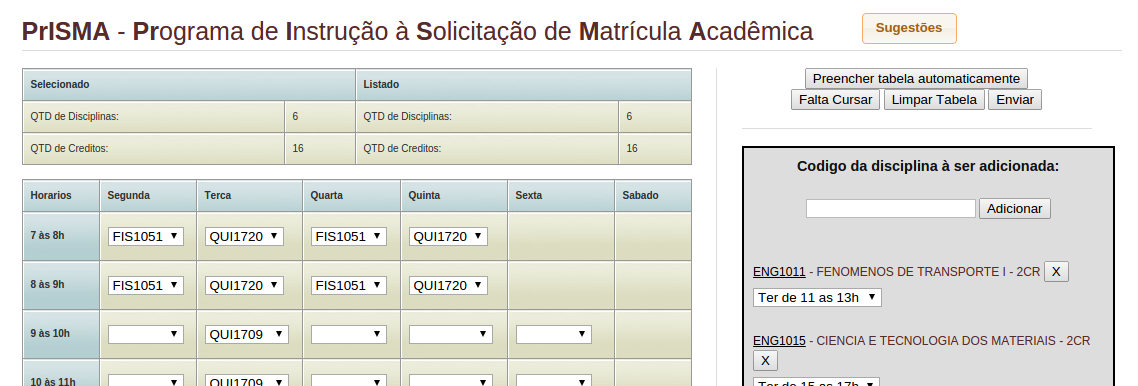
\includegraphics[width=\linewidth]{img/v2_horario.png}
    \caption{Tela principal.}
\end{figure}

Passada essa etapa. Apresenta-se então uma tela de resultado final, apresentando as turmas selecionadas como primeira opção, e demais turmas da mesma disciplina como demais opções. Essa heurística utilizada não é a melhor, no entanto, continua sendo uma abordagem válida.

\begin{figure}[H]
    \centering
    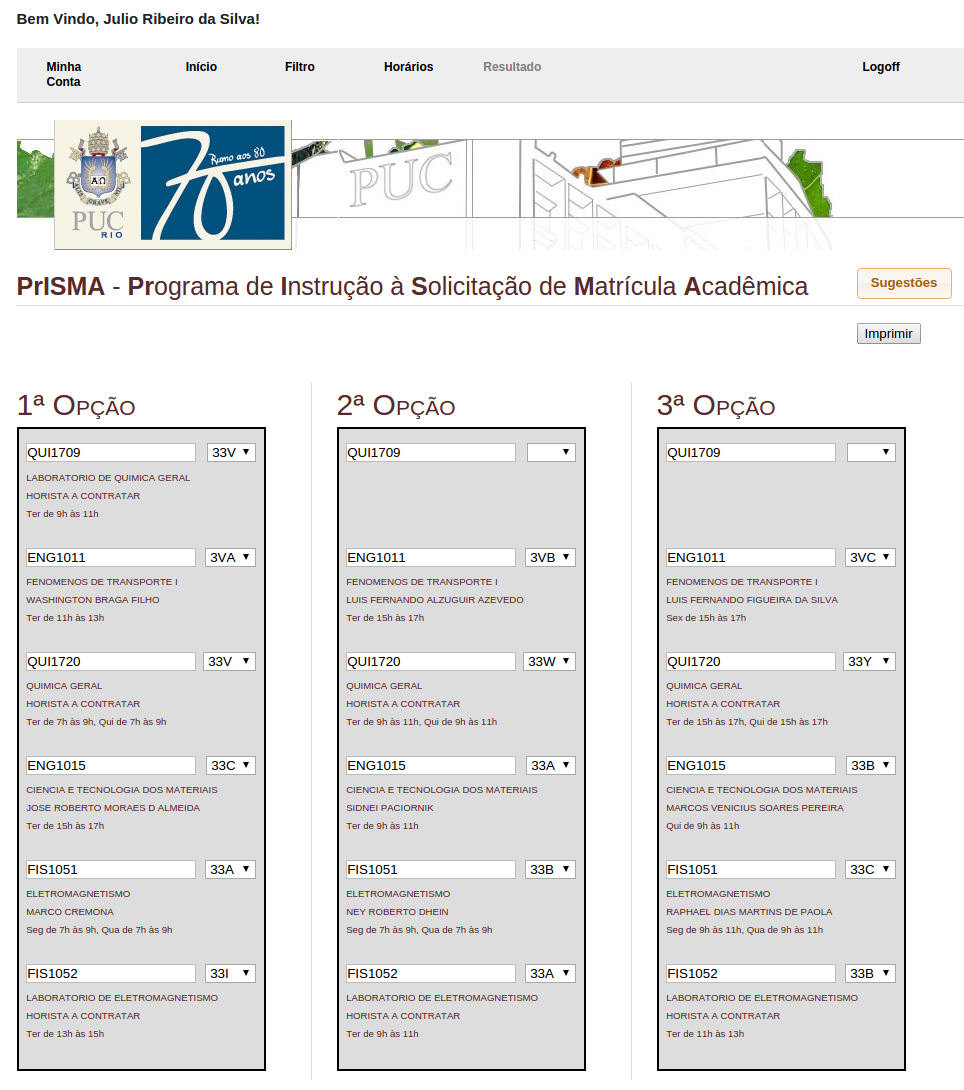
\includegraphics[width=\linewidth]{img/v2_final.png}
    \caption{Tela de resultado final.}
\end{figure}

Essa versão, por mais que ainda estivesse bastante limitada as funcionalidades apresentadas na versão anterior, já atendia uma parcela considerável das necessidades dos alunos.  


\section{Versão final}

Por conta das limitações das versões anteriores e pela baixa manutenibilidade do código gerado nas versões anteriores, decidiu-se por implementar uma versão completamente nova do PrISMA, tirando proveito de toda experiência adquirida até então e todos os feedbacks recebidos.

Foi então que um grupo do curso de design, da PUC-Rio, apresentou um conceito que abordava o mesmo contexto trabalhado, com uma preocupação muito maior a aparência da solução, facilidade de uso e disponibilidade dos dados e ferramentas de apoio à tomada de decisão.

\begin{figure}[H]
    \centering
    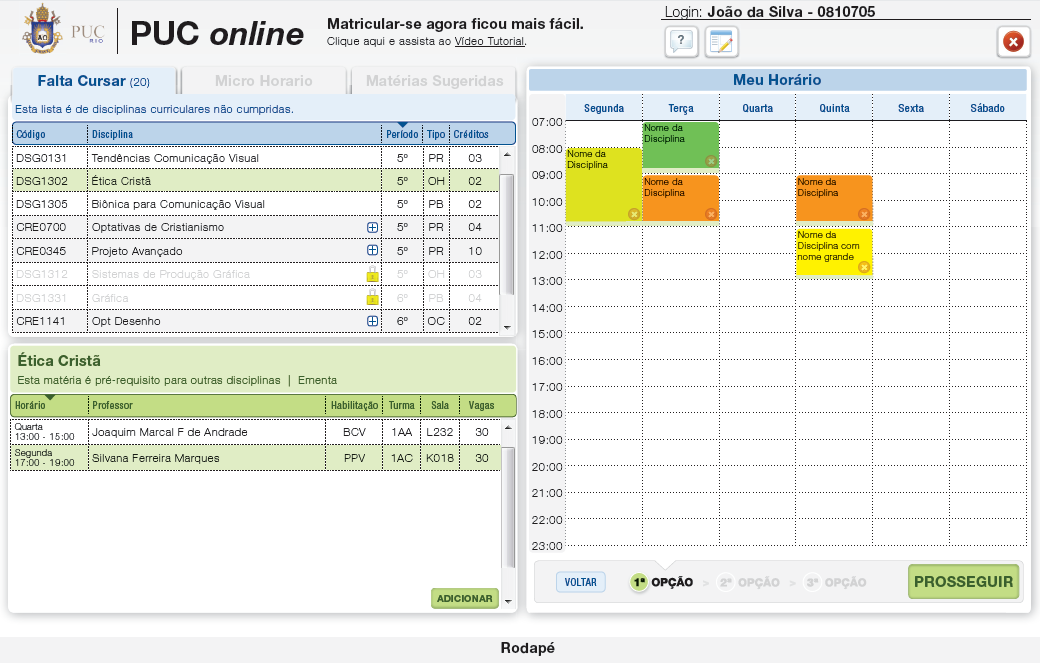
\includegraphics[width=\linewidth]{img/designer.png}
    \caption{Versão conceitual.}
\end{figure}

Com esta versão, as disciplinas a serem escolhidas ficam no lado esquerdo da tela, separando por abas aquelas pertencentes ao Falta-Cursar, as buscadas diretamente no Micro-Horário e aquelas que seriam sugeridas pelo sistema, de maneira automática. No lado direito se encontram as disciplinas selecionadas, sendo uma tabela para cada opção, como pode-se notar na parte inferior da tela.

Nesse ponto, foi notado que tanto a versão antiga, quanto esse conceito novo se completavam. Visualmente a interface do conceito se adequa bem melhor ao problema. As disciplinas sugeridas foram deixadas de lado, por demandar de uma inteligência que não seria viável de se implementar no momento, e no seu lugar foram inseridas as disciplinas selecionadas, desta vez no mesmo formato do sistema antigo do PUC Online, em referência à lista de disciplinas selecionadas na versão anterior do PrISMA. Da mesma maneira, mais possibilidades de interação foram adicionadas ao conceito, como será visto mais para frente.

\begin{figure}[H]
    \centering
    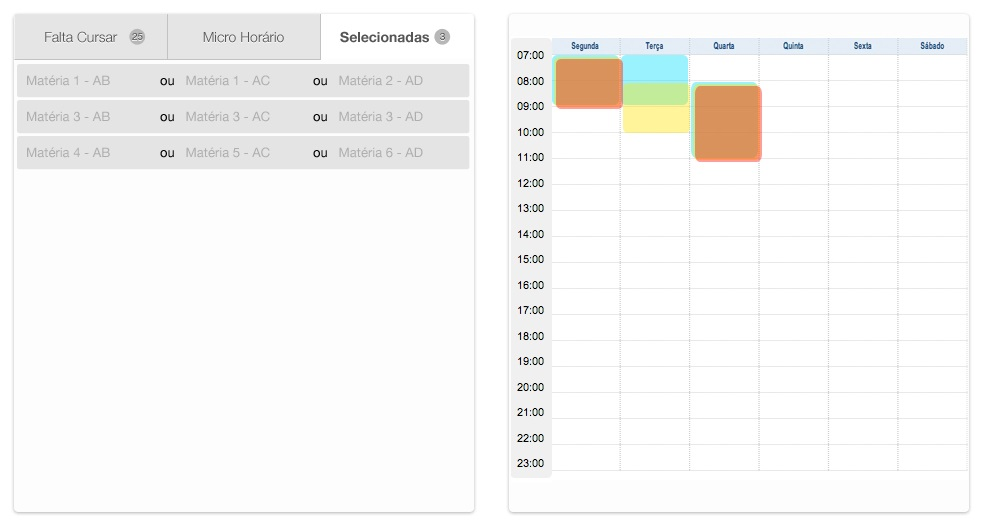
\includegraphics[width=\linewidth]{img/prisma-WF.jpg}
    \caption{União entre conceito e o PrISMA.}
\end{figure}

Nesta etapa, ainda não se sabia como seriam de fato representadas as opções no sistema. Na aba de selecionadas as disciplinas já seriam exibidas no mesmo formato esperado pelo sistema da PUC, mas na tabela de horários a visualização de diversas turmas, uma em cima da outra, poderia ficar bastante confusa.

Foi aí então que entrou a funcionalidade de simulação na combinação das turmas. Ficou acordado que na tabela de horários não seria exibida mais de uma turma no mesmo horário e que, essa combinação exibida seria, na verdade, o resultado de uma simulação ocorrida na aba de selecionadas. Essa simulação se refere exatamente ao comportamento definido pelo processamento das turmas pelo sistema da PUC. Isto é, as primeiras turmas e primeiras opções tem prioridades sobre as outras. Logo, uma vez selecionadas, os horários se tornariam indisponíveis para as próximas. 
Visto que a quantidade de combinações possíveis nessa simulação cresce exponencialmente, no primeiro momento apenas a primeira solução é apresentada, de maneira gulosa, assim como o algoritmo apresentado na primeira versão do PrISMA. No entanto, desta vez, pode-se marcar alguma opção especifica como sendo selecionada, para que seja possível visualizar a consequência nas demais turmas a serem solicitadas. E da mesma forma, a combinação simulada será apresentada na tabela de horários do lado direito.

\begin{figure}[H]
    \centering
    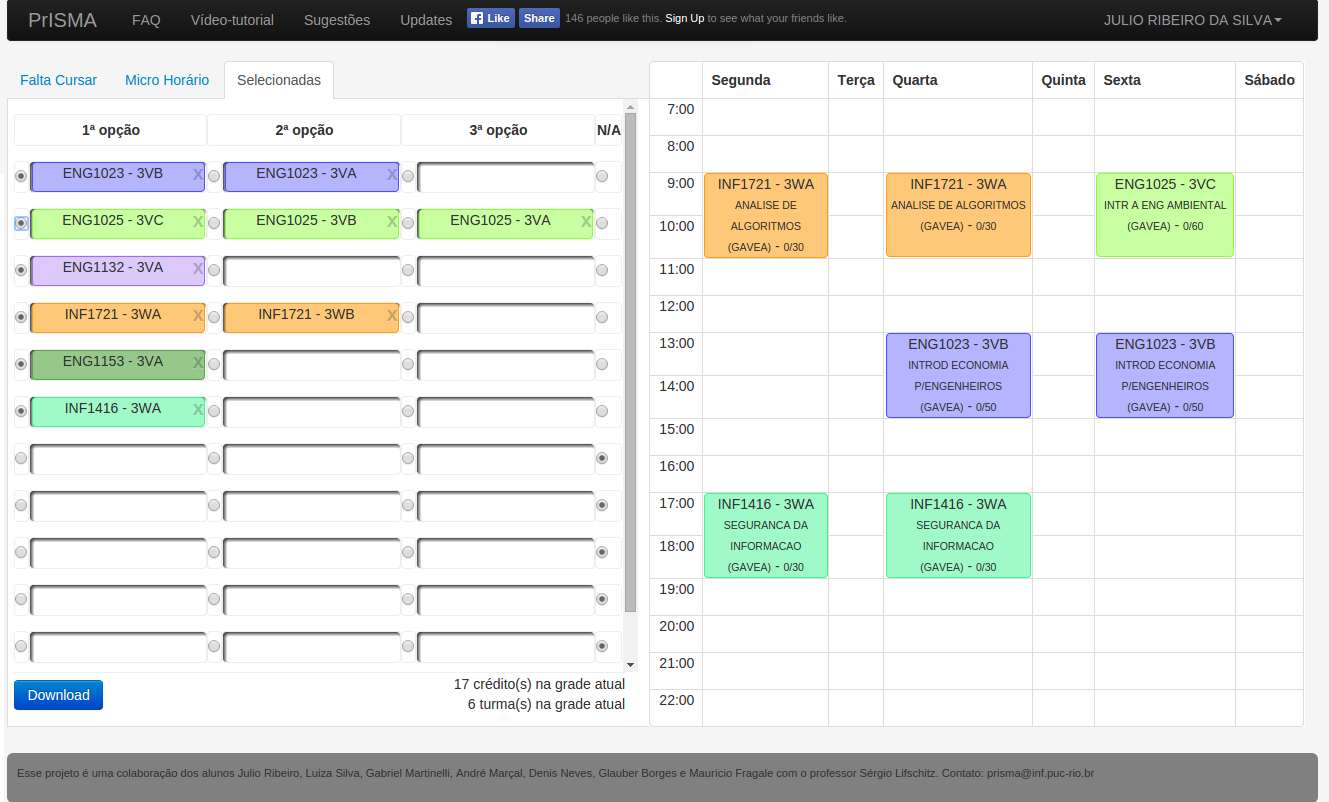
\includegraphics[width=\linewidth]{img/v3_selecionadas.png}
    \caption{Versão final do PrISMA - aba selecionadas.}
\end{figure}

As demais abas continuaram bastante parecidas com o conceito inicial proposto pelos designers. A única modificação foi a identidade de cores e os campos de busca na aba de Micro-Horário.

\begin{figure}[H]
    \centering
    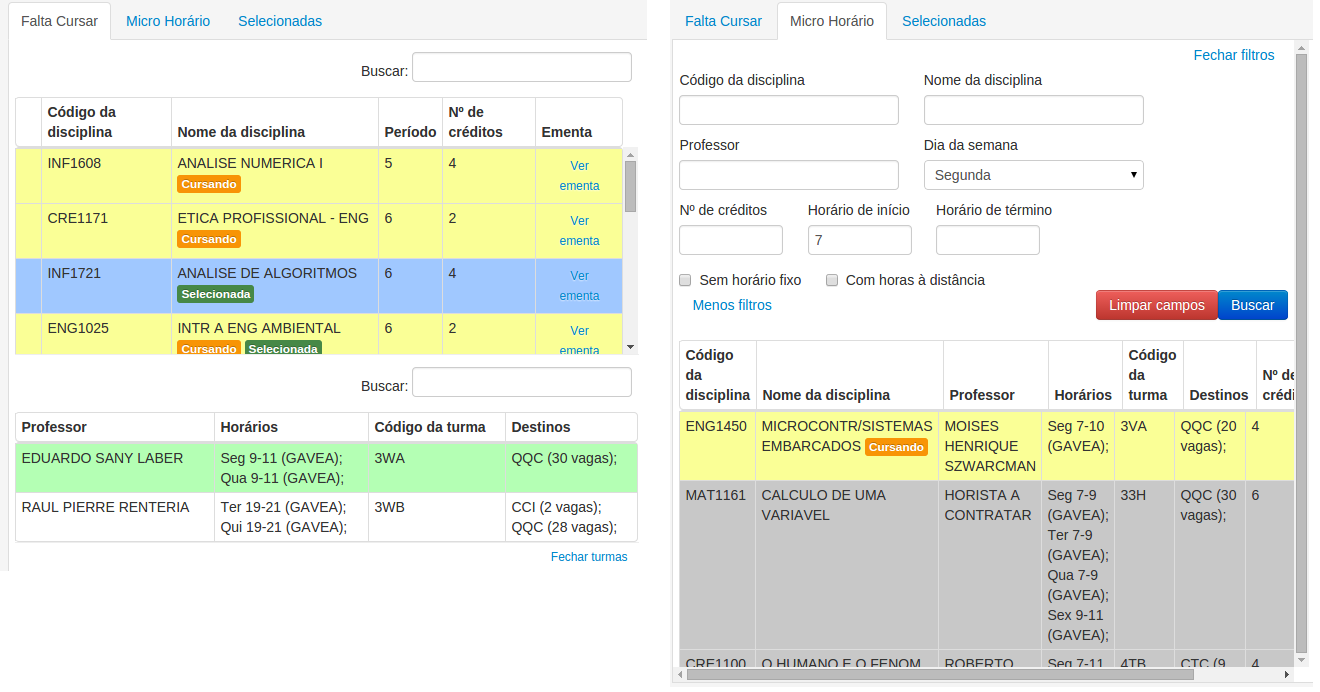
\includegraphics[width=\linewidth]{img/v3_abas.png}
    \caption{Versão final do PrISMA - aba Falta-Cursar e Micro-Horário.}
\end{figure}

Diversas outras funcionalidades foram implementas, conforme segue:

\begin{itemize}

	\item Ao selecionar uma disciplina, uma notificação aparece ao lado da aba de disciplinas selecionadas para o usuário saber que ocorreu uma alteração foi corretamente processada.
	\item Na aba Falta-Cursar, são exibidas todas as disciplinas do Falta-Cursar. No entanto, aquelas que estão sendo cursadas no período corrente aparecem em amarelo, as que estão presas por pré-requisitos aparecem em vermelho e as demais em branco.
	\item Na aba de Micro-Horário, as disciplinas encontradas que já foram cursadas aparecem em cinza.
	\item Tanto na aba de Falta-Cursar quanto de Micro-Horário, aquelas turmas que já foram selecionadas ou estão sendo cursadas aparecem com uma mensagem informando essas situações.
	\item Ao clicar em uma célula vazia na tabela de horários, é realizada uma busca pelas turmas que estão sendo disponibilizadas naquele horário clicado.
	\item Ao clicar em uma turma, na tabela de horários, é realizada uma busca no Micro-Horário pelas demais turmas daquela respectiva disciplina clicada.
	\item Para exportar o resultado final, basta clicar no botão de download, na aba de disciplinas selecionadas.
	\item No cabeçalho do sistema são disponibilizados FAQ, um \href{https://www.youtube.com/watch?v=XHF8WOJ6xI0}{vídeo} com explicação do sistema e uma área para feedbacks.

\end{itemize}

Para este projeto final, foram implementadas também as funcionalidades de estatísticas de uso, pra ser usado como feedback para os responsáveis pelos departamentos, download do resultado final e feedback para o aluno quanto à sua classificação frente àqueles que também solicitaram a mesma turma.

Esse último recurso, de feedback ao aluno, foi implementado recentemente e por conta disso não foi disponibilizado para os alunos. Ele pode ser visualizado na tabela de horários, na célula referente a cada turma. Ali encontra-se um número seguido de uma barra, seguida de outro número. O primeiro indica a classificação do aluno frente aos demais da turma e o segundo indica a quantidade de vagas disponíveis para aquela turma. Dessa forma, os alunos podem se planejar melhor também quanto ao seu ranking perante a PUC.

Quanto à forma de acesso ao sistema, foi dispensado o cadastro individual de cada aluno e passou-se a utilizar as próprias credencias utilizadas no PUC Online. Da mesma forma, todos os dados dos alunos, como falta-cursar, histórico e disciplinas que estão sendo cursadas no momento foram disponibilizadas diretamente ao sistema, mediante termo de confidencialidade. Dessa maneira, foi possível realizar a checagem dos pré-requisitos para cada disciplina, para cada aluno, e eliminar a etapa de cadastro.


%%%%%%%%%%%%%%%%%%%%%%%%%%%%%%%%%%%%%%%%%%%%%%%%%%%%%%%%%%%%%%%%%%%%%%%%%%%%%%%%

\chapter{Implementação}

Nesta seção serão abordados os aspectos técnicos da última versão implementada do PrISMA, assim como as decisões quanto ferramentas e padrões que foram adotados. As versões mais antigas não serão abordadas por terem sido implementadas sem grandes preocupações com a Engenharia de Software em si, se tratando apenas de uma etapa introdutória ao mundo do desenvolvimento Web.

A solução é baseada em uma aplicação Web. Isto é, existe um servidor com o objetivo de persistir e compilar os dados que serão apresentados aos usuários, e apenas os seus dados. E existe uma aplicação que é executava no navegador dos usuários, que utiliza extensivamente de requisições dinâmicas de forma que seja reduzido ao máximo o tráfego de dados e, consequentemente a carga no servidor, e as transições dentro da aplicação fiquem mais suaves a ponto de se aproximem mais de uma aplicação desktop.

O servidor utilizado para hospedar o projeto foi disponibilizado pelo Sérgio Lifschitz que, com a ajuda do suporte do Departamento de Informática (principalmente o Anderson Oliveira da Silva), foi relacionado com o domínio “prisma.inf.puc-rio.br”. A configuração utilizada no servidor foi a distribuição TurnKey, com servidor Apache, servidor PostgreSQL e pacotes para que seja possível a execução de scripts em PHP. Na configuração final fez-se uso de SSL, sem a disponibilidade de certificado validado por Autoridade Certificadora.

Todo código gerado foi versionado utilizando-se GIT e hospedado na plataforma \href{https://github.com/PrismaDev/prisma}{GitHub}. Sendo open-source, todos podem contribuir, usar como referência ou mesmo reutilizar projeto como um todo.

O padrão MVC (Model-view-controller) foi utilizado duas vezes na implementação do sistema. Uma no lado do servidor (back-end), outra no lado do aplicativo que é executado no navegador (front-end). A comunicação entre essas duas camadas se dá por intermédio dos respectivos controllers, utilizando requisições dinâmicas e o formato JSON para transmissão dos dados.

\section{Banco de Dados}

Nas primeiras versões foi utilizado o SGBD MySQL para persistência e consistência dos dados. Na última versão, o PostgreSQL. A mudança foi realizada por conta do último ter melhor desempenho, ser mais rico em funcionalidades e ter a preferência dos desenvolvedores.

Abaixo será explicado todo o modelo desenvolvido, assim como as decisões tomadas.

\subsection{Tabelas}

Utilizando a ferramenta DbVisualizer foi possível gerar o seguinte diagrama de tabelas e relacionamentos:

\begin{figure}[H]
    \centering
    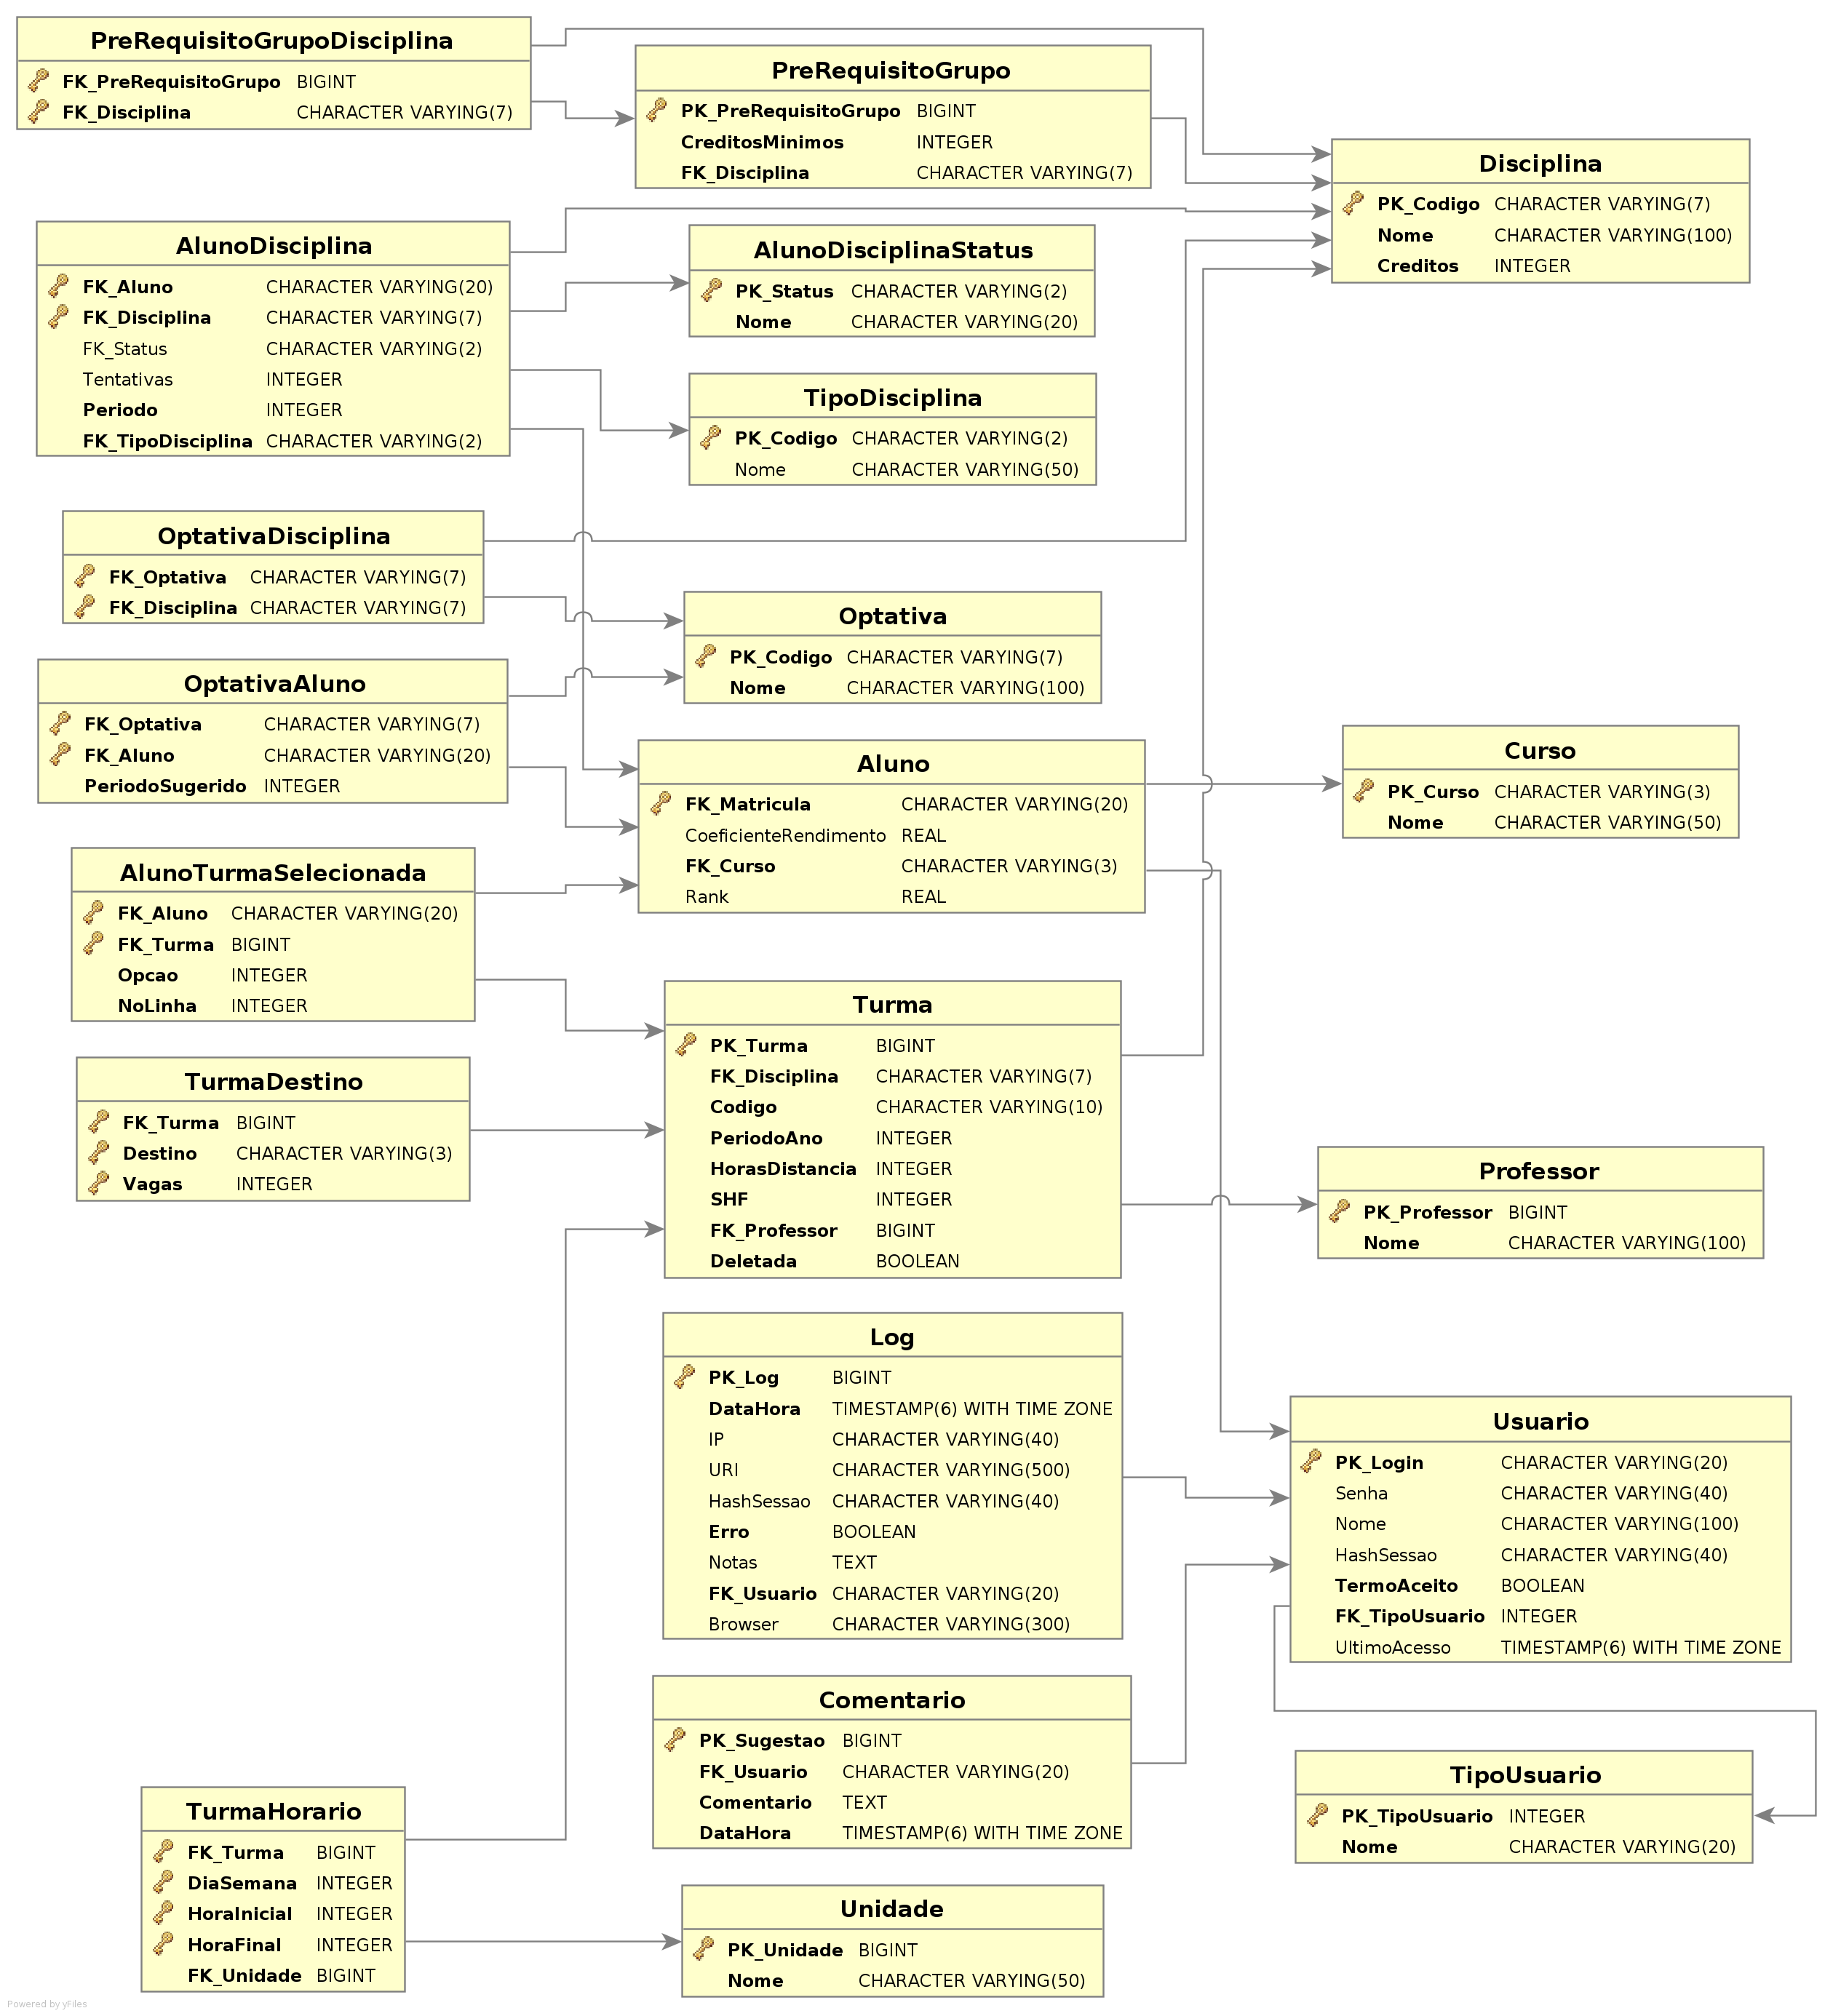
\includegraphics[width=\linewidth]{img/dbvisualizer.png}
    \caption{Modelo Relacional do Banco de Dados.}
\end{figure}

Com base no modelo acima, segue a descrição de cada tabela:

\begin{itemize}

	\item \underline{Aluno}: é um tipo de usuário no sistema, no caso, aquele que realizará a escolha de turmas para montar sua grade;
	\begin{itemize}
		\item FK\_Matrícula: referência login do usuário que, quando aluno, é a sua matrícula;
		\item CoeficienteRendimento: coeficiente de rendimento do aluno acumulado;
		\item FK\_Curso: referência para o curso do aluno;
		\item Rank: valor utilizado para classificar alunos de acordo com sua prioridade na hora de fazer suas escolhas.
	\end{itemize}

	\item \underline{AlunoDisciplina}: representa o relacionamento de um aluno com disciplina;
	\begin{itemize}
		\item FK\_Aluno: referência para Aluno;
		\item FK\_Disciplina: referência para disciplina;
		\item FK\_Status: reference para AlunoDisciplinaStatus;
		\item Tentativas: quantidade de vezes que aluno tentou cursar uma turma desta disciplina;
		\item Periodo: Caso a disciplina tenha sido cursada alguma vez, se trata do período que foi cursada pela última vez. Caso contrário, se trata do período sugerido para ser cursada, caso obrigatória;
		\item FK\_TipoDisciplina: referência para TipoDisciplina;
	\end{itemize}

	\item \underline{AlunoDisciplinaStatus}: tabela estática que explicita quais Status são possíveis. Possui as tuplas (CP, cumpriu), (EA, em andamento) e (NC, não cumpriu);
	\begin{itemize}
		\item PK\_Status: identificador único
		\item Nome: descrição do Status;
	\end{itemize}

	\item \underline{AlunoTurmaSelecionada}: relaciona Aluno com Turma, representando as escolhas feitas pelos alunos;
	\begin{itemize}
		\item FK\_Aluno:  referência para o Aluno;
		\item FK\_Turma: referência para a Turma;
		\item Opcao: opção referente à tabela de entrada de dados, no modelo antigo do PUC Online;
		\item NoLinha: número da linha referente à tabela de entrada de dados, no modelo antigo do PUC Online;
	\end{itemize}

	\item \underline{Comentário}: armazena as sugestões feitas pelos usuários;
	\begin{itemize}
		\item PK\_Sugestão: identificador único gerado automaticamente;
		\item FK\_Usuario: referência para o Usuário que fez a sugestão;
		\item Comentário: texto que representa o comentário em si;
		\item DataHora: data e hora que o comentário foi feito;
	\end{itemize}

	\item \underline{Curso}: registra os diferentes cursos de graduação que podem ser cursados pelos Alunos;
	\begin{itemize}
		\item PK\_Curso: identificador único;
		\item Nome: nome do curso;
	\end{itemize}

	\item \underline{Disciplina}: representa uma disciplina;
	\begin{itemize}
		\item PK\_Codigo: identificador único composto por 3 letras e 4 números;
		\item Nome: nome da disciplina;
		\item Creditos: quantidade de créditos que o aluno acumulará ao cumprir a disciplina;
	\end{itemize}

	\item \underline{Log}: registra toda interação feita pelo usuário;
	\begin{itemize}
		\item PK\_Log: identificador único gerado automaticamente;
		\item DataHora: data e hora do registro;
		\item IP: endereço IP do usuário que gerou o log;
		\item URI: endereço relacionado à requisição feita pelo usuário;
		\item HashSessao: identificador da sessão do usuário;
		\item Erro: indica se foi registrado algum erro no processamento da requisição;
		\item Notas: texto detalhando o erro ou anormalidade constatada;
		\item FK\_Usuario: referência ao Usuário;
		\item Browser: informa qual navegador foi utilizado ao efetuar a requisição;
	\end{itemize}

	\item \underline{Optativa}: representa um grupo de optativas (obrigatoriedade de cursar ao menos uma disciplina pertencente ao grupo);
	\begin{itemize}
		\item PK\_Codigo: identificador do grupo de optativa, composto por 3 letras e 4 números;
		\item Nome: nome do grupo de optativa;
	\end{itemize}

	\item \underline{OptativaAluno}: parte do Falta-Cursar, onde é definido quais optativas os Alunos devem cursar;
	\begin{itemize}
		\item FK\_Optativa: referência para Optativa;
		\item FK\_Aluno: referência para Aluno;
		\item PeriodoSugerido: período sugerido para que seja cursada pelo Aluno;
	\end{itemize}

	\item \underline{OptativaDisciplina}: relaciona Optativa com Disciplina, informando quais disciplinas compõem o grupo de optativas;
	\begin{itemize}
		\item FK\_Optativa: referência para Optativa;
		\item FK\_Disciplina: referência para Disciplina;
		\item FK\_Optativa: referência para Optativa;
	\end{itemize}

	\item \underline{PreRequisitoGrupo}: cada disciplina ter mais de um grupo relacionado. Para que o pré-requisito para uma disciplina seja validado, apenas um grupo precisa ser atendido. Isto é, todas as disciplinas do grupo sejam cursadas e a quantidade mínima de créditos atendida;
	\begin{itemize}
		\item PK\_PreRequisitoGrupo: identificador único gerado automaticamente;
		\item CreditosMinimos: quantidade mínima de créditos acumulados pelos Alunos para que este grupo seja atendido;
		\item FK\_Disciplina: referência para a Disciplina que possui este pré-requisito;
	\end{itemize}

	\item \underline{PreRequisitoGrupoDisciplina}: disciplinas que compõem um grupo de pré-requisito. Todas devem ser cursadas para que o grupo de pré-requisito seja atendido;
	\begin{itemize}
		\item FK\_PreRequisitoGrupo: referência para PreRequisitoGrupo;
		\item FK\_Disciplina: referência para disciplina que faz parte do grupo;
	\end{itemize}

	\item \underline{Professor}: representa os professores;
	\begin{itemize}
		\item PK\_Professor: identificador único gerado automaticamente;
		\item Nome: nome do professor;
	\end{itemize}

	\item \underline{TipoDisciplina}: tabela estática que informa se disciplina do Falta-Cursar é eletiva, optativa, obrigatória, etc.;
	\begin{itemize}
		\item PK\_Codigo: identificador único;
		\item Nome: descrição;
	\end{itemize}

	\item \underline{TipoUsuário}: tabela estática que informa qual o tipo de usuário. Pode ser administrador, aluno, etc;
	\begin{itemize}
		\item PK\_TipoUsuario: identificador único
		\item Nome: descrição;
	\end{itemize}

	\item \underline{Turma}: representa uma turma. Deve, obrigatoriamente, ter um professor relacionado;
	\begin{itemize}
		\item PK\_Turma: identificador único gerado automaticamente;
		\item FK\_Disciplina: referência à disciplina correspondente;
		\item Codigo: código composto por 3 caracteres alfanuméricos, que identificam a turma para cada disciplina;
		\item PeriodoAno: período e ano que a turma está sendo oferecida;
		\item HorasDistancia: quantidade de horas semanais que a turma exige que seja cumprida a distância (sem sala de aula);
		\item SHF: sem horário fixo;
		\item FK\_Professor: referência para o professor relacionado;
		\item Deletada: booleano que invalida turma;
	\end{itemize}

	\item \underline{TurmaDestino}: a quantidade de vagas de uma turma pode ser reservada para diferentes cursos;
	\begin{itemize}
		\item FK\_Turma: referência para Turma;
		\item Destino: código do destino (Destino não modelado, este código é apenas exibido para o aluno);
		\item Vagas: quantidade de vagas reservadas ao destino relacionado;
	\end{itemize}

	\item \underline{TurmaHorario}: relaciona as Turmas com seus respectivos horários de aula;
	\begin{itemize}
		\item FK\_Turma: referência para Turma;
		\item DiaSemana: inteiro identificando o dia da semana;
		\item HoraInicial: inteiro identificando hora de início da aula;
		\item HoraFinal: inteiro identificando hora de término da aula;
		\item FK\_Unidade: campus da universidade onde a turma é ministrada;
	\end{itemize}

	\item \underline{Unidade}: representa diferentes campus da universidade;
	\begin{itemize}
		\item PK\_Unidade: identificador único gerado automaticamente;
		\item Nome: nome do local onde fica localizado o campus;
	\end{itemize}

	\item \underline{Usuário}: representa um usuário;
	\begin{itemize}
		\item PK\_Login: representa o login do usuário no sistema;
		\item Senha: MD5 da senha do usuário;
		\item Nome: nome do usuário;
		\item HashSessao: identificador único de sessão do usuário. É atualizado a cada novo login. É necessário para efeito para o log;
		\item TermoAceito: variável booleana que indica aceitação do termo de compromisso para utilização do sistema. Caso não seja aceito, o acesso não é concedido.
		\item FK\_TipoUsuario: define se usuário é Aluno, Administrador, etc.;
		\item UltimoAcesso: data e hora do último login do usuário;
	\end{itemize}

\end{itemize}

\subsection{Visões}

\begin{itemize}
	\item \underline{AlunoDisciplinaTurmaSelecionada}: para cada disciplina selecionada para o aluno, também retorna a quantidade total de vagas e a quantidade de alunos que também selecionaram esta Turma, mas que tem classificação superior ao Aluno corrente no ranking da PUC-Rio. Não inclui turmas que tenham sido deletadas;
	\item \underline{EstatisticaDemandaHorario}: para cada horário, conta-se a quantidade de alunos que tenham escolhido uma turma neste respectivo horário;
	\item \underline{EstatisticaDemandaTurma}: conta quantos alunos escolheram determinada Turma. Informa também a quantidade de vagas disponível;
	\item \underline{FaltaCursarOptativa}: retorna apenas as optativas que fazem parte do Falta-Cursar. Isto é, que ainda não tenham sido completadas;
	\item \underline{FaltaCursarOptativaDisciplina}: para as optativas que fazem parte do Falta-Cursar, informa as disciplinas que compõem o grupo e a situação dos Alunos frente a elas. Isto é, se estão cursando e/ou se estão aptos a cursá-las;
	\item \underline{LogAcessoSegundo}: estatística de acesso ao sistema, por segundo. Conta cada requisição realizada pelos Usuários;
	\item \underline{LogAlunoAno}: estatística que informa a quantidade de alunos que acessaram o sistema, agrupado pelo ano de entrada na universidade;
	\item \underline{LogAlunoCurso}: estatística quanto ao percentual de alunos que acessaram o sistema, por curso. Isto é, informa qual é a quantidade total de alunos por curso e a quantidade que efetivamente fez uso do sistema;
	\item \underline{LogAlunoSelecionada}: estatística que informa a quantidade de alunos que selecionaram ao menos uma Turma e a quantidade média de turmas selecionadas por eles;
	\item \underline{LogErro}: se trata apenas da tabela de log filtrada pelo atributo Erro, que indica quando ocorreu algum erro inesperado;
	\item \underline{LogHistogramaBrowserUsuario}: estatística que informa quantos usuários utilizaram os diferentes navegadores existentes;
	\item \underline{LogQuantidadeUsuario}: estatística que informa a quantidade de usuários que acessaram o sistema ao menos uma vez;
	\item \underline{LogUsuarioAcesso}: conta quantas vezes cada usuario acessou o sistema e, utilizando esse valor, agrupa-se os usuarios que acessaram a mesma quantidade de vezes e realiza a contagem, para cada quantidade de acesso;
	\item \underline{LogUsuarioDia}: quantidades de usuários únicos que acessaram o sistema, por dia;
	\item \underline{MicroHorario}: recupera o Micro-Horário original, realizando a união das tabelas Disciplinas, Turmas, Professor, TurmaHorario e TurmaDestino;
	\item \underline{MicroHorarioDisciplina}: para cada Aluno e para cada Disciplina, informa se já foi cursada e/ou está apta a ser cursada;
	\item \underline{TurmaHorarioUnidade}: união entre TurmaHorario e TurmaUnidade apenas;
	\item \underline{TurmaProfessor}: união entre Turma e Professor, apenas;
	\item \underline{UsuarioAluno}: relacionamento entre Usuario e Aluno, apenas;
\end{itemize}

\subsection{Visões}

As funções abstraem consultas que são realizadas por diferentes visões, ou mesmo outras funções, ou que são mais complexas que as demais. São elas:

\begin{itemize}
	\item \underline{AlunoCreditos( $<$MatriculaAluno$>$, $<$StatusSituacao$>$ )}: conta a quantidade de créditos cursados pelo aluno que tenham  cujas disciplinas tenham a situação passada por parâmetro. Caso a situação seja NC (não cumpriu), considera-se apenas as disciplinas do Falta-Cursar;
	\item \underline{AlunoCreditosCursados( $<$MatriculaAluno )}: análoga à função anterior, só que apenas para disciplinas que tenham status CP (cumpriu);
	\item \underline{AlunoDisciplinaApto( $<$MatriculaAluno$>$, $<$CodigoDisciplina$>$ )}: para este par Aluno-Disciplina, verifica-se se ele atende todos os pré-requisitos para cursar a dada disciplina. Caso retorno seja 2, pode cursar. Caso 1, cuidado, disciplina está sendo cursada ou quantidade de créditos necessário para cursá-la depende das suas aprovações no período corrente. Caso 0, presa por pré-requisito. Para cada par Aluno-Disciplina, verifica-se se há algum grupo de pré-requisito que seja composto apenas por disciplinas que já tenham sido cumpridas;
	\item \underline{AlunoDisciplinaSituacao( $<$MatriculaAluno$>$, $<$CodigoDisciplina$>$ )}: para cada Aluno e Disciplina, informa situação. Isto é, se foi cumprida, se está em andamento ou se não foi cumprida;
	\item \underline{AlunoOptativaCursada( $<$MatriculaAluno$>$, $<$CodigoOptativa$>$ )}: para cada Optativa que deve ser cursada pelo Aluno, verifica-se se há pelo menos uma Disciplina deste grupo que tenha sido cumprida pelo Aluno;
	\item \underline{AlunoTurmaRank( $<$MatriculaAluno$>$, $<$IdTurma$>$ )}: para cada Turma selecionada por um Aluno, conta quantos alunos que também selecionaram aquela Turma tem classificação maior do que o Aluno referenciado;
	\item \underline{DisciplinaTemPrequisito( $<$CodigoDisciplina$>$ )}: apenas informa se existe referência à dada disciplina na tabela PreRequisitoGrupo;
	\item \underline{LimpaBanco()}: limpa banco de dados, sem zerar tabelas estáticas;
	\item \underline{TurmaVagasTotal( $<$IdTurma$>$ )}: para a dada Turma, informa a quantidade de vagas total que está sendo oferecida;
\end{itemize}


\section{Aplicação do servidor}

As requisições efetuadas por cada cliente são direcionadas ao servidor para uma porta e um IP específico. Esta porta deve ter sido previamente aberta por um servidor HTTP, que estará esperando as conexões dos clientes. Esse servidor, por sua vez, deve encaminhar as requisições para a aplicação para que sejam devidamente respondidas.

A aplicação, neste caso, foi escrita em PHP. Para auxiliar no desenvolvimento da aplicação, foi utilizado o framework Very Simple PHP Rest Framework, desenvolvimento especialmente para este projeto.

\subsection{Alternativas}

\paragraph{Servidor HTTP}

Diversos outros servidores HTTP estão disponíveis, no entanto nenhum é tão utilizado e reconhecido quanto o da Apache. Este se demonstra muito fácil de ser configurado e já vem instalado em grande parte das distribuições UNIX.

\paragraph{Linguagem da aplicação}

A linguagem PHP tem uma grande vantagem de ter uma curva de aprendizado muito suave, principalmente pra quem já sabe programar em outras linguagens como Java e C. Dessa forma, por conta de maior domínio dos programadores, e pelo problema não exigir nenhuma operação muito complexa que precisasse ser otimizada, por conveniência foi escolhido o PHP mesmo.

\paragraph{Framework}

Diversos frameworks estão disponíveis em PHP. Dentre eles: Zend Framework, Symfony, CakePHP, etc. No entanto, todos apresentam muitas funcionalidades e cada um tem a sua forma de lidar com a organização do projeto em si. 

Por conta disso, e visando também o aprendizado sobre como funciona um framework, foi desenvolvido um framework especificamente para este projeto, o Very Simple PHP Rest Framework. Que se trata de um framework bastante minimalista, que lida apenas com o correto direcionamento das requisições para os devidos controles, controla a conexão com o banco de dados e lida com o processamento de templates.


\subsection{Framework utilizado}

Nesta seção será explicada a organização dos arquivos da aplicação no servidor e como ocorre o fluxo de dados.

Quando o servidor HTTP encaminha uma requisição para a aplicação, tendo sempre a raiz do projeto como referência, ele irá olhar para a pasta “$<$root$>$/Public” e verificar se existe algum arquivo, inclusive em subpastas, com o nome especificado pela URL. Caso não exista, a requisição será encaminhada para o arquivo “index.php”, nesta própria pasta. Dessa maneira, o framework iniciará o seu tratamento.

Todo da aplicação fica localizado em uma pasta que não é “visível” pelo Apache. Isso é, os arquivos não podem ser acessados diretamente por uma URL. Essa pasta é “$<$root$>$/Application”. Dentro dela, na pasta “Config” estão os arquivos de configuração da aplicação. Dentre eles a configuração de conexão com o banco de dados e os arquivos que faz o mapeamento de URL com controllers.

Na pasta “Prisma” está fica a aplicação em si. Essa pasta faz uso do padrão MVC. Onde o model é são apenas interfaces de comunicação com o banco de dados, representando assim cada entidade do modelo apresentado anteriormente. A visão é representada por todo elemento que será enviado ao browser para exibição do conteúdo. O controller contém todo código responsável por responder as requisições.

Como o framework faz uso do padrão Orientação Objeto, para se criar um controller basta que ele seja mapeado no arquivo de configuração, relacionando assim com uma URL, e estenda a classe RestController, que se encontra no módulo “Framework”.

Cada controller inclui os modelos necessários para interfaceamento com o banco de dados e responde com o que foi solicitado. A resposta pode ser um conjunto de dados no formato JSON ou uma página Web.

\subsection{Configuração do ambiente}

Na pasta “$<$root$>$/Documents” tem um arquivo chamado “installation.txt”, que aponta os comandos a serem executados em ambientes Debian, a fim de realizar a correta instalação do sistema. Este arquivo pode ser usado como referência para outros ambientes também.

\section{Front-end}

O PrISMA é dividido basicamente em três páginas, do ponto de vista do servidor. A primeira é a página de login, a segunda é a página de termo de compromisso e a última a página da aplicação em si. Vale ressaltar que as duas últimas só são acessíveis caso haja um usuário logado como aluno. E a última, por sua vez, só é acessível caso o termo de compromisso tenha sido aceito.

Na tentativa de minimizar ao máximo a tranferencia de dados entre o cliente e o servidor, diversas técnicas e ferramentas foram utilizadas. Como, por exemplo, minimizar todo arquivo Javascript, CSS e HTML enviado. Essa minimização consiste em remover todo caracter considerado nulo ou substituir palavras por outras menores, sem que haja qualquer alteração na informação a ser transmitida.

A página da aplicação, por mais que seja apenas uma, possui muita funcionalidade e, vez ou outra, precisa persistir ou recuperar dados do servidor. Para que a página inteira não seja recarregada, foram utilizadas requisições dinâmica (Ajax), transferindo sempre dados no formato JSON.

Diversas ferramentas foram utilizadas para auxiliar no desenvolvimento e na construção da aplicação a ser executava no navegador, tanto do lado do servidor quanto do cliente.

\subsection{Desenvolvimento}

Na pasta “$<$root$>$/Application/Prisma/View” estão todos os arquivos necessários para desenvolvimento do front-end, e os templates que serão processados pelo servidor e fornecidos ao navegador. Estes templates tem extensão “.ptml” e se encontram na raiz. Eles também são gerados automaticamente.

No navegador também é utilizado o padrão MVC. Neste caso, este padrão é implementado pela ferramenta Backbone, conforme pode ser visto na pasta “js-dev”. Para cada interação realizada na aplicação no navegador, existe uma rotina implementada em um controle da pasta “controller”. Um modelo similar ao banco de dados é implementado na pasta “model”, para que seja mais fácil de ser acessar e organizar os dados. E na pasta “view” fica todo controle responsável pela montagem do que será exibido ao usuário. Foi utilizada a ferramenta Closure, da Google, para compilação e minimização destes arquivos de controle.

Quando o servidor entrega ao navegador os dados no primeiro momento, não se trata de uma página pronta para ser exibida. O controle da aplicação se encarregará de unir os templates recebidos com os dados e organizá-los corretamente. O processamento dos templates no lado do cliente é feita pela ferramenta Underscore.

Para auxiliar no desenvolvimento da interface foi utilizado como base a biblioteca Bootstrap. Nele já são definidos diversos elementos que são altamente customizáveis, tanto em termo de comportamento quanto de estilo em si.

Os elementos de estilo se encontram na pasta “less-dev”. Less é uma ferramenta bastante poderosa que adiciona diversas funcionalidade ao CSS. O código gerado passa por uma etapa de compilação para que seja gerado o CSS final. Cada arquivo nessa pasta representa um módulo da aplicação.

Para facilitar a geração da estrutura dos templates foi utilizada a ferramenta Jade. Com essa ferramenta é aumentar consideravelmente a produtividade. E no final o arquivo gerado é um HTML devidamente minimizado. Na pasta “phtml-jade-dev” estão os templates que serão processados pelo servidor. Na pasta “template-jade-dev” estão os templates que serão processados pelo Underscore, no cliente.

Cara página, do ponto de vista do servidor, tem um arquivo Javascript e um arquivo CSS associados. Esses arquivos são gerados a partir de todos aqueles vistos anteriormente. Para auxiliar essa geração foi utilizada a ferramenta GNU Make. Dessa maneira o processo de desenvolvimento fica completamente automatizado.

Na pasta “$<$root$>$/Public” estão as pastas “css”, “js” e “img”, que contém todos aqueles arquivos que serão providos ao navegador de forma estática. Isto é, não são modificados para cada requisição. Os arquivos CSS e Javascript ali contidos já são aqueles processados e devidamente minimizados, conforme visto anteriormente.

\chapter{Resultado}

Fazer parte do desenvolvimento do PrISMA foi um grande prazer, e é motivo de muito orgulho, dado que foi utilizado como base para o novo sistema do PUC Online.

A primeira versão do prisma disponibilizada foi disponibilizada nos primeiros e segundos semestres de 2011 e 2012. A segunda versão foi disponibilizada nos primeiros e segundos semestres de 2013 e apenas no primeiro semestre de 2014. Quando a PUC-Rio parou de oferecer suporte por entender que o sistema não era mais necessário, por conta do novo sistema desenvolvido pela equipe do SAU, par o PUC Online.

O PrISMA foi utilizado, em média, por 1500 alunos em um único período, chegando ao pico de 2400, no segundo semestre do ano de 2013. Isto é, entre 10\% e 20\% dos total de alunos da PUC-Rio. Segundo o Washington Brava, diretor do DAR, foi notada uma sutil melhora na qualidade das solicitações realizadas.

Em suma, este sistema se demonstrou bastante útil para o planejamento da vida acadêmica dos alunos de graduação. E, por se tratar de um problema tão difícil de ser resolvido, que teve que ser contornado por meio diversas ferramentas de apoio, o resultado se demonstra bastante positivo.


\chapter{Trabalhos futuros}

Conforme foi visto, o sistema desenvolvido teve uma excelente aceitação, mas algumas funcionalidades ainda podem ser adicionadas.

A primeira delas é a integração oficial com o sistema do PUC Online, de forma que o aluno não precise se planejar em um ambiente, e entrar com os dados oficialmente em outro.

Atualmente, para cada período novo, alguns cuidados devem ser tomados na hora de importar os dados. Se faz necessário a criação de uma página de administrador, onde seria possível avaliar todo o comportamento do sistema, assim como inserir e remover usuários que não sejam alunos.

As estatísticas estão devidamente implementadas, mas poderiam ser melhor direcionadas para quem está visualizando. Neste caso, deveria haver conta de coordenador de departamento, que teria acesso à todos os dados referentes aos seus cursos.

Deveria ser possível adicionar e remover turmas diretamente no PrISMA, enquanto está sendo utilizado pelos alunos. Essa necessidade que aparece naturalmente ao visualizar as estatísticas e constatar que a oferta de turmas não condiz com a demanda.

No mesmo contexto do problema dos alunos, diversas ferramentas poderiam ser utilizadas para auxiliar o coordenador na hora de organizar as turmas a serem oferecidas. Da mesma forma, poderia haver um mapeamento de salas e disponibilidades de professores, assim como as disciplinas que podem ser ministradas por eles.

E, para finalizar, resolver pequenos problemas de implementação e refinar as funcionalidades já implementadas.

%%%%%%%%%%%%%%%%%%%%%%%%%%%%%%%%%%%%%%%%%%%%%%%%%%%%%%%%%%%%%%%%%%%%%%%%%%%%%%%%
\arial
\nocite{*}
\bibliography{relatorio2}

\normalfont

% \appendix
% \includepdf[pages=-]{ArtigoLuiza.pdf}

\end{document}
